% latex article template

% cheat sheet(eng): http://www.pvv.ntnu.no/~walle/latex/dokumentasjon/latexsheet.pdf
% cheat sheet2(eng): http://www.pvv.ntnu.no/~walle/latex/dokumentasjon/LaTeX-cheat-sheet.pdf
% reference manual(eng): http://ctan.uib.no/info/latex2e-help-texinfo/latex2e.html

% The document class defines the type of document. Presentation, article, letter, etc. 
\documentclass[12pt, a4paper]{article}

% packages to be used. needed to use images and such things. 
\usepackage[pdfborder=0 0 0]{hyperref}
\usepackage[utf8]{inputenc}
\usepackage[english]{babel}
\usepackage{graphicx}
\PassOptionsToPackage{hyphens}{url}

% hides the section numbering. 
\setcounter{secnumdepth}{-1}

% Graphics/image lications and extensions. 
\DeclareGraphicsExtensions{.pdf, .png, .jpg, .jpeg}
\graphicspath{{./images/}}

\title{
	Architectural Design Document \\
    TDT4240 - Group A14 \\
	~\\
	\normalsize{
	\underline{Framework:} \\ 
	Android\\
    ~\\
	\underline{Quality Attributes:} \\
	Primary: Modifiability \\
	Secondary: Useability \\ 
    ~\\
	}
}
\author{
	\underline{Group members:} \\
    Bremnes, Jan A. S.\\
    Johanessen, Stig Tore\\
	Hesselberg, Håkon \\
    Kirø, Magnus L.\\
	Randby, Simon \\
    Tørresen, Håvard\\
}
\date{\today}

\hypersetup{
	colorlinks=true,
	linkcolor=black,
	filecolor=red,
	urlcolor=blue
}

\begin{document}
\maketitle
\pagenumbering{arabic}

\newpage
\tableofcontents
\newpage

\section{Introduction}

\subsection{Project description}
The overall lines of the project are to create a game for Android. In the process of creating the game there are some document requirements that has to be fulfilled before we can create the game. This document is this prephase for the actual development of the game. 

Our game concept is based on the classic Battleship. We are going to recreate it and make room for improvements and further expansion of the game concept. We plan a first version that has basic functionality, where we focus on the architecture, modularity and expandability. When the first version is complete we will expand the functionality to implement extensions like different types of ammunition, different ships, varying number of missiles, etc. 

Another idea we will look into is ship levels and experience. Increasing firepower, speed and other properties after winning battles. 

The game can also be expanded to incorporate a turn based network addition. 

\subsection{Document structure}
This document contains all the relevant aspects of the architectural design for the game that we are going to create. We introduce our game concept and document structure in the introduction. 

Continuing with requirements of the architecture and an overview of stakeholders and concerns that we have. 

Then the architecture is described with views, tactics, design patterns and a rationale of the architecture.

At the end we cover issues, references and changes. 

\subsection{Phase(requirement)}
The current phase of the project is the requirements specification and design specification. The whole point of this phase is to create goals that we will reach in the implementation phase. Goals will help us to keep on track and have progress. 


\section{Architectural Drivers/Architectural Significant Requirements}

The main drivers in the project, aka the most important aspects of the development process. 

\subsection{Delivery Deadline}
It’s always important to keep deadlines. This one is no exception. It will also become very busy for everyone as the semester draws to an end. People have excursions and other subjects have projects. We expect that this will not become a problem, since we will structure our work accordingly.

\subsection{Code completion / working game}

Getting a working code base and a game is important. To have a working result the code has to compile and function. This also includes that we have implemented working aspects of our game idea. 

\section{Extendability}

The extendability of the code base is one of the more important factors. This is specified by the course and we find it very important as this is the fun part of the project. 

\section{Stakeholders and concerns}
\begin{itemize}
	\item \textit{Stakeholder}
	\subitem \textit{Concerns}
\end{itemize}

\begin{itemize}
	\item Players
	\subitem The usability of the game, the gameplay and the evolution of possibilities 

	\item Developers
	\subitem Code extensibility, code convention, readability, 

	\item Teaching assistants
	\subitem Code quality, readability, functionality, documentation

	\item Future employers
	\subitem End result. 
\end{itemize}

\section{Selection of Architectural views}

\begin{itemize}
	\item Logical view
	\subitem \textbf{Purpose:} Object model of the design
	\subitem \textbf{Stakeholders:} Developers, ATAM evaluators, course staff.
	\subitem \textbf{Form of description:} Class diagram

	\item Process view
	\subitem \textbf{Purpose:} Capture concurrency and synchronization aspects
	\subitem \textbf{Stakeholders:} Developers, ATAM evaluators, course staff
	\subitem \textbf{Form of description:} Activity diagrams

	\item Development view
	\subitem \textbf{Purpose:} Static organisation of software in its development environment
	\subitem \textbf{Stakeholders:} Developers, ATAM evaluators, course staff
	\subitem \textbf{Form of description:} Architecture layer diagram

\end{itemize}


\section{Architecturail tactics}

Our main focus in terms of quality requirements will be modifiability of the code, something which both of our design patterns are known for being capable of achieving. MVC is traditionally easy to implement and easy to understand when modifying the code. It also allows for easy switching of the graphical system of the application, without touching the game logic. On the other end of modifiability we have the configuration options provided by using abstract factories together with XML files to provide configurable game experience and content.

Our secondary focus will be on usability. While our design patterns do not directly support this as of yet, the use of MVC means that the user interface and design can easily be changed without having to alter how the game works. This should hopefully provide us with ample opportunity to customise the user experience.

Unfortunately both our primary and secondary quality requirements are near impossible to quantify, so any quantifiable quality will focus on our quality requirements list. Most of these quality requirements are focused around the reliability of the app, which is heavily supported by our choice of design patterns. The reliability of the app will depend much our concurrence with the patterns and by following best practices of the programing language. 


\section{Architectural and design pattern}
We’re planning to utilise MVC and Abstract Factory Patterns in our architectural design. 

MVC to separate functionality, design and data. Keep the logic in one place, the user interface another and add send the data objects between them. 

The abstract factory pattern will be used to ease the use of different game types. This will enable us to have multiple game modes easily available through different implementations of base factories. 

\section{Views}
The views we have selected are, as mentioned above, a logical, a process and a development view. They are supported by the various diagrams shown below:

% imgae example. 
\begin{figure}[H]
    \centering
    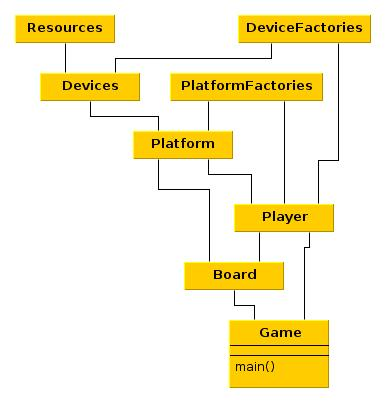
\includegraphics[width=\textwidth]{over}
    \caption{The class diagram shows how we imagine the different classes we need, and their connections.
}
    \label{fig:over}
\end{figure}
    
% imgae example. 
\begin{figure}[H]
    \centering
    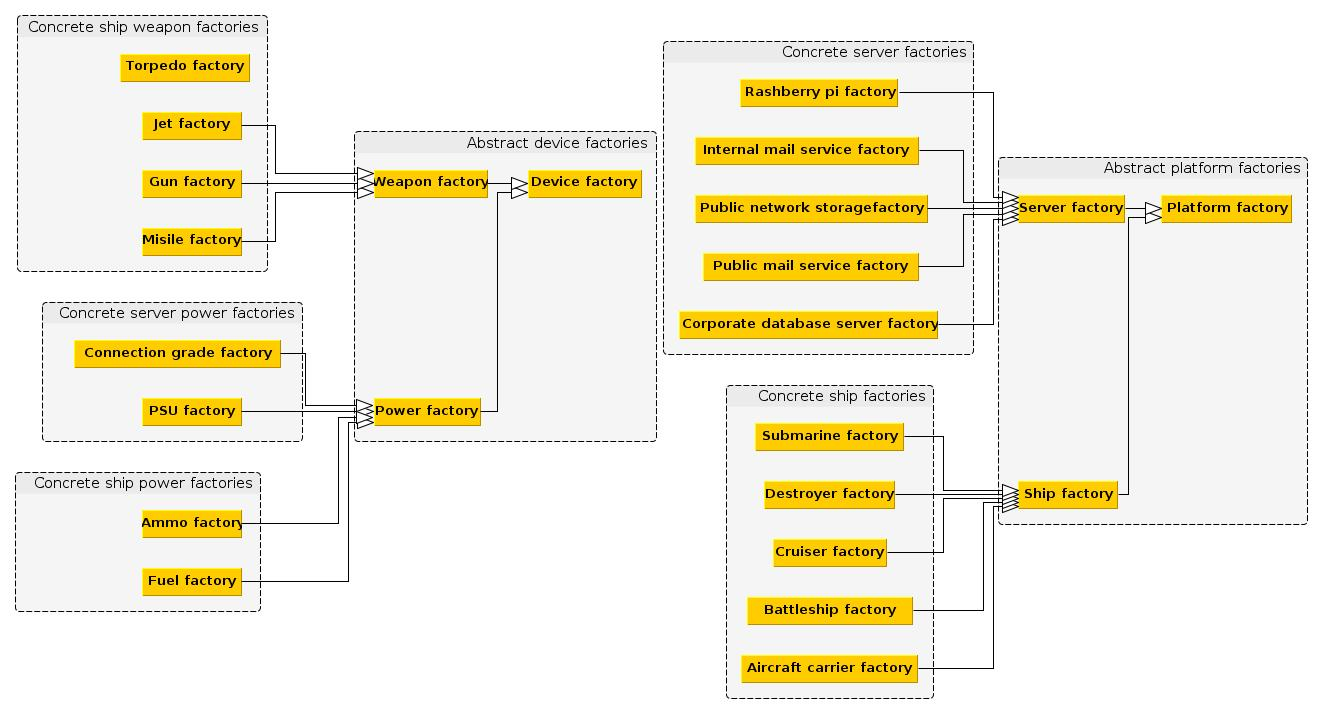
\includegraphics[width=\textwidth]{klasse}
    \caption{The class diagram shows how we imagine the different classes we need, and their connections.
}
    \label{fig:klasse}
\end{figure}

% imgae example. 
\begin{figure}[H]
    \centering
    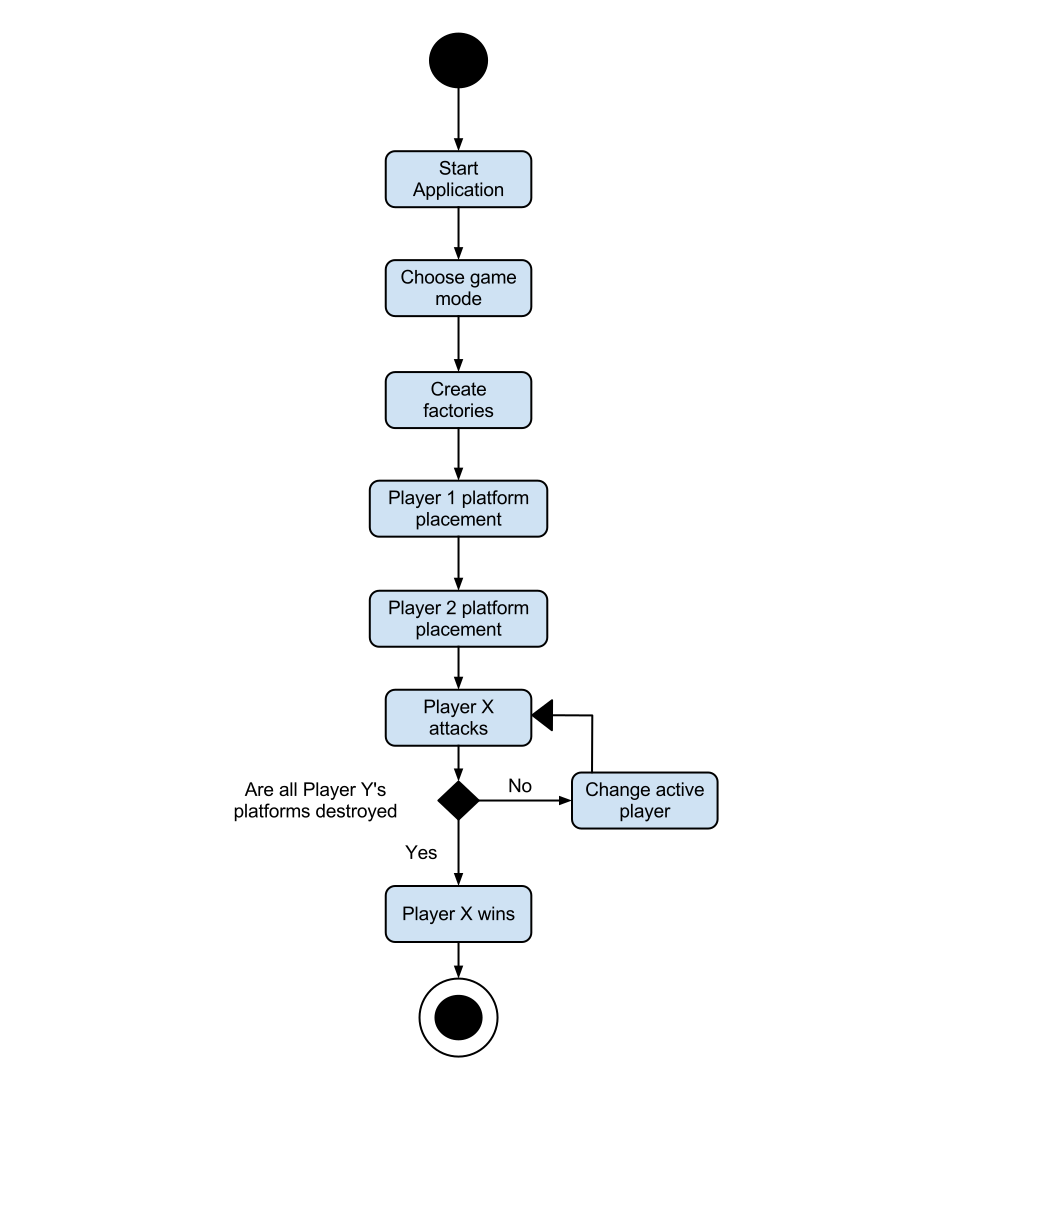
\includegraphics[width=\textwidth]{activity}
    \caption{The activity diagram shows the flow of actions from the application start to the end of the game.}
    \label{fig:activity}
\end{figure}

% imgae example. 
\begin{figure}[H]
    \centering
    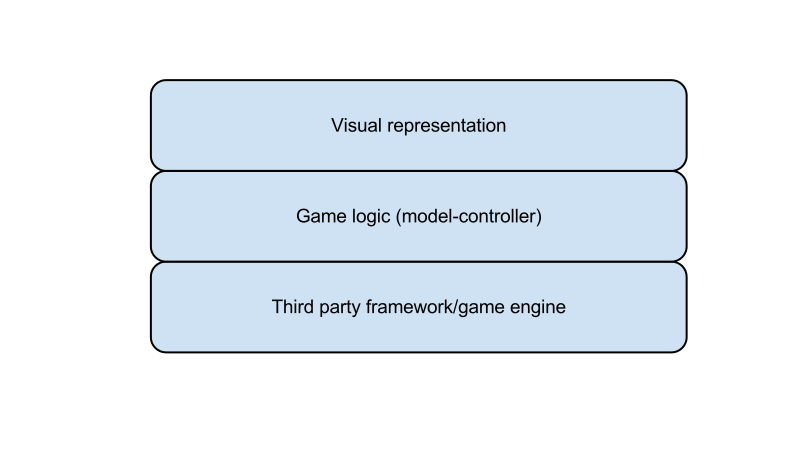
\includegraphics[width=\textwidth]{arch}
    \caption{The architecture layer diagram shows how the application is divided into layers.
}
    \label{fig:arch}
\end{figure}

\section{Consistency among views}
We have not found any inconsistencies among the views, if we did they would have been taken care of. 

\section{Architectural Rationale}
The choice to use MVC is based on its common use, and it’s history of modifiability, reliability and ease of coding.

Abstract factories configured using XML came as a natural choice, as this will allow us to easily extend the game. 

\section{Issues}
We were debating whether to use the abstract factory pattern or method factories. We decided abstract factories looked like they would allow for far greater modifiability while not leading to a much more complex implementation.

\section{References}
Abstract Factory Design Pattern; Web: \url{http://www.lepus.org.uk/ref/companion/AbstractFactory.xml} Accessed 2013-03-04.

\section{Changes}
None. 

\end{document}
